% Options for packages loaded elsewhere
\PassOptionsToPackage{unicode}{hyperref}
\PassOptionsToPackage{hyphens}{url}
\PassOptionsToPackage{dvipsnames,svgnames*,x11names*}{xcolor}
%
\documentclass[
  english,
  man,floatsintext]{apa6}
\usepackage{lmodern}
\usepackage{amssymb,amsmath}
\usepackage{ifxetex,ifluatex}
\ifnum 0\ifxetex 1\fi\ifluatex 1\fi=0 % if pdftex
  \usepackage[T1]{fontenc}
  \usepackage[utf8]{inputenc}
  \usepackage{textcomp} % provide euro and other symbols
\else % if luatex or xetex
  \usepackage{unicode-math}
  \defaultfontfeatures{Scale=MatchLowercase}
  \defaultfontfeatures[\rmfamily]{Ligatures=TeX,Scale=1}
\fi
% Use upquote if available, for straight quotes in verbatim environments
\IfFileExists{upquote.sty}{\usepackage{upquote}}{}
\IfFileExists{microtype.sty}{% use microtype if available
  \usepackage[]{microtype}
  \UseMicrotypeSet[protrusion]{basicmath} % disable protrusion for tt fonts
}{}
\makeatletter
\@ifundefined{KOMAClassName}{% if non-KOMA class
  \IfFileExists{parskip.sty}{%
    \usepackage{parskip}
  }{% else
    \setlength{\parindent}{0pt}
    \setlength{\parskip}{6pt plus 2pt minus 1pt}}
}{% if KOMA class
  \KOMAoptions{parskip=half}}
\makeatother
\usepackage{xcolor}
\IfFileExists{xurl.sty}{\usepackage{xurl}}{} % add URL line breaks if available
\IfFileExists{bookmark.sty}{\usepackage{bookmark}}{\usepackage{hyperref}}
\hypersetup{
  pdftitle={Epidemiologische situatie COVID-19 in Nederland - 10 december 2021},
  pdfauthor={Marino van Zelst1},
  pdflang={en-EN},
  colorlinks=true,
  linkcolor=Maroon,
  filecolor=Maroon,
  citecolor=Blue,
  urlcolor=blue,
  pdfcreator={LaTeX via pandoc}}
\urlstyle{same} % disable monospaced font for URLs
\usepackage{graphicx,grffile}
\makeatletter
\def\maxwidth{\ifdim\Gin@nat@width>\linewidth\linewidth\else\Gin@nat@width\fi}
\def\maxheight{\ifdim\Gin@nat@height>\textheight\textheight\else\Gin@nat@height\fi}
\makeatother
% Scale images if necessary, so that they will not overflow the page
% margins by default, and it is still possible to overwrite the defaults
% using explicit options in \includegraphics[width, height, ...]{}
\setkeys{Gin}{width=\maxwidth,height=\maxheight,keepaspectratio}
% Set default figure placement to htbp
\makeatletter
\def\fps@figure{htbp}
\makeatother
\setlength{\emergencystretch}{3em} % prevent overfull lines
\providecommand{\tightlist}{%
  \setlength{\itemsep}{0pt}\setlength{\parskip}{0pt}}
\setcounter{secnumdepth}{-\maxdimen} % remove section numbering
% Make \paragraph and \subparagraph free-standing
\ifx\paragraph\undefined\else
  \let\oldparagraph\paragraph
  \renewcommand{\paragraph}[1]{\oldparagraph{#1}\mbox{}}
\fi
\ifx\subparagraph\undefined\else
  \let\oldsubparagraph\subparagraph
  \renewcommand{\subparagraph}[1]{\oldsubparagraph{#1}\mbox{}}
\fi
% Manuscript styling
\usepackage{upgreek}
\captionsetup{font=singlespacing,justification=justified}

% Table formatting
\usepackage{longtable}
\usepackage{lscape}
% \usepackage[counterclockwise]{rotating}   % Landscape page setup for large tables
\usepackage{multirow}		% Table styling
\usepackage{tabularx}		% Control Column width
\usepackage[flushleft]{threeparttable}	% Allows for three part tables with a specified notes section
\usepackage{threeparttablex}            % Lets threeparttable work with longtable

% Create new environments so endfloat can handle them
% \newenvironment{ltable}
%   {\begin{landscape}\begin{center}\begin{threeparttable}}
%   {\end{threeparttable}\end{center}\end{landscape}}
\newenvironment{lltable}{\begin{landscape}\begin{center}\begin{ThreePartTable}}{\end{ThreePartTable}\end{center}\end{landscape}}

% Enables adjusting longtable caption width to table width
% Solution found at http://golatex.de/longtable-mit-caption-so-breit-wie-die-tabelle-t15767.html
\makeatletter
\newcommand\LastLTentrywidth{1em}
\newlength\longtablewidth
\setlength{\longtablewidth}{1in}
\newcommand{\getlongtablewidth}{\begingroup \ifcsname LT@\roman{LT@tables}\endcsname \global\longtablewidth=0pt \renewcommand{\LT@entry}[2]{\global\advance\longtablewidth by ##2\relax\gdef\LastLTentrywidth{##2}}\@nameuse{LT@\roman{LT@tables}} \fi \endgroup}

% \setlength{\parindent}{0.5in}
% \setlength{\parskip}{0pt plus 0pt minus 0pt}

% \usepackage{etoolbox}
\makeatletter
\patchcmd{\HyOrg@maketitle}
  {\section{\normalfont\normalsize\abstractname}}
  {\section*{\normalfont\normalsize\abstractname}}
  {}{\typeout{Failed to patch abstract.}}
\patchcmd{\HyOrg@maketitle}
  {\section{\protect\normalfont{\@title}}}
  {\section*{\protect\normalfont{\@title}}}
  {}{\typeout{Failed to patch title.}}
\makeatother
\shorttitle{Dagelijkse rapportage}
\DeclareDelayedFloatFlavor{ThreePartTable}{table}
\DeclareDelayedFloatFlavor{lltable}{table}
\DeclareDelayedFloatFlavor*{longtable}{table}
\makeatletter
\renewcommand{\efloat@iwrite}[1]{\immediate\expandafter\protected@write\csname efloat@post#1\endcsname{}}
\makeatother
\usepackage{csquotes}
\ifxetex
  % Load polyglossia as late as possible: uses bidi with RTL langages (e.g. Hebrew, Arabic)
  \usepackage{polyglossia}
  \setmainlanguage[]{english}
\else
  \usepackage[shorthands=off,main=english]{babel}
\fi

\title{Epidemiologische situatie COVID-19 in Nederland - 10 december 2021}
\author{Marino van Zelst\textsuperscript{1}}
\date{}


\affiliation{\vspace{0.5cm}\textsuperscript{1} Vragen over deze rapportage kunnen verstuurd worden aan Marino van Zelst, twitter.com/mzelst. E-mail: \href{mailto:j.m.vanzelst@uvt.nl}{\nolinkurl{j.m.vanzelst@uvt.nl}}}

\begin{document}
\maketitle

{
\hypersetup{linkcolor=}
\setcounter{tocdepth}{3}
\tableofcontents
}
\newpage

\hypertarget{samenvatting}{%
\section{Samenvatting}\label{samenvatting}}

\textbf{Samenvatting (op basis van GGD cijfers)}\\
Tot en met 2021-12-10 zijn er in Nederland in totaal 2846126 COVID-19 patiënten gemeld aan het RIVM. Tot nu toe zijn 36421 van de gemelde patiënten opgenomen in het ziekenhuis en 20004 mensen overleden.

\textbf{Gegevens t. o. v. gisteren}\\
Positief getest: 17562
Totaal: 2846126 (+ 17471 ivm -91 corr.)

Opgenomen: 96
Totaal: 36421 (+
94 ivm -2 corr.)

Overleden: 85
Totaal: 20004 (+
85 ivm 0 corr.)

\textbf{Update met betrekking tot ziekenhuis-gegevens (data NICE)}

Patiënten verpleegafdeling\\
Bevestigd: 19 Verdacht: 5

Patiënten IC\\
Bevestigd: 11 Verdacht: 0

\textbf{Data}\\
Een databestand met de cumulatieve aantallen per gemeente per dag van gemelde COVID-19 patiënten, in het ziekenhuis opgenomen COVID-19 patiënten en overleden COVID-19 patiënten is \href{https://data.rivm.nl/geonetwork/srv/dut/catalog.search\#/metadata/1c0fcd57-1102-4620-9cfa-441e93ea5604}{hier} te vinden. Een databestand met karakteristieken van elke positief geteste COVID-19 patiënt in Nederland is \href{https://data.rivm.nl/geonetwork/srv/dut/catalog.search\#/metadata/2c4357c8-76e4-4662-9574-1deb8a73f724?tab=relations}{hier} te vinden. Alle gegevens die voor dit rapport gebruikt worden zijn te vinden in de \href{https://github.com/mzelst/covid-19}{Github repository}.

\newpage

\hypertarget{covid-19-meldingen-in-de-afgelopen-vier-weken}{%
\section{COVID-19 meldingen in de afgelopen vier weken}\label{covid-19-meldingen-in-de-afgelopen-vier-weken}}

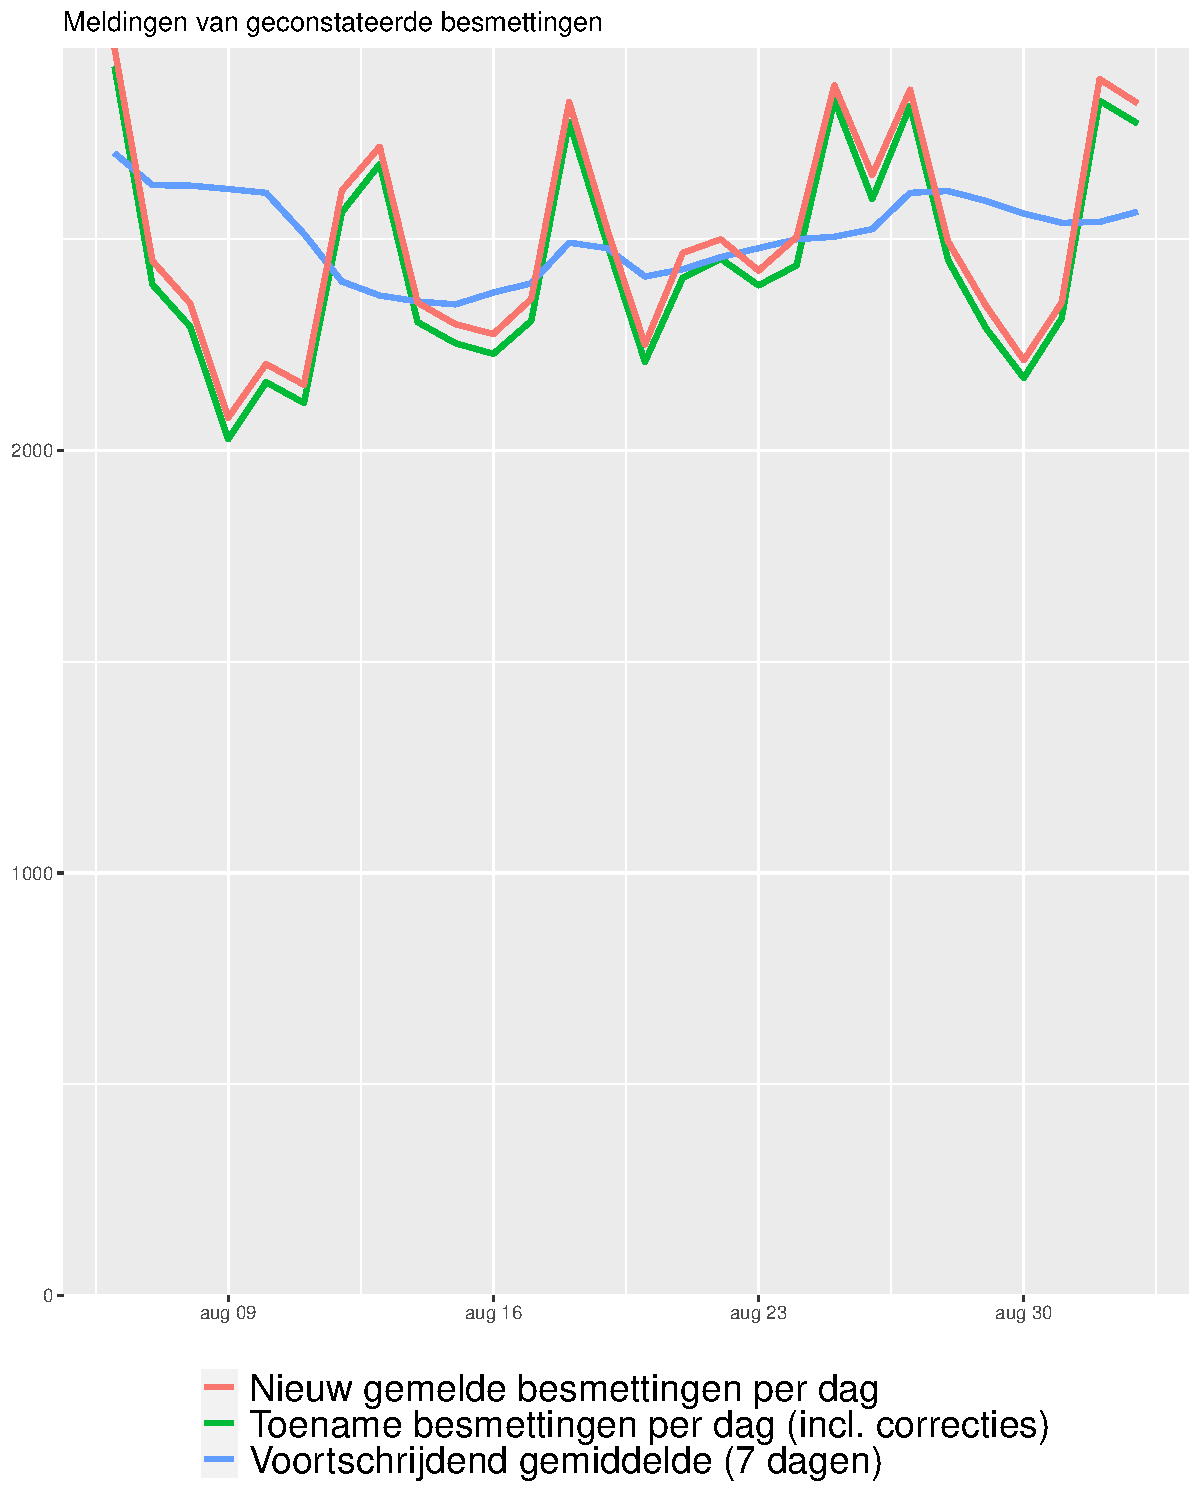
\includegraphics{daily_report_files/figure-latex/Gemelde besmettingen-1.pdf}

\newpage

\hypertarget{kaart-met-covid-19-meldingen-per-gemeente-sinds-gisteren}{%
\section{Kaart met COVID-19 meldingen per gemeente sinds gisteren}\label{kaart-met-covid-19-meldingen-per-gemeente-sinds-gisteren}}

\begin{figure}
\centering
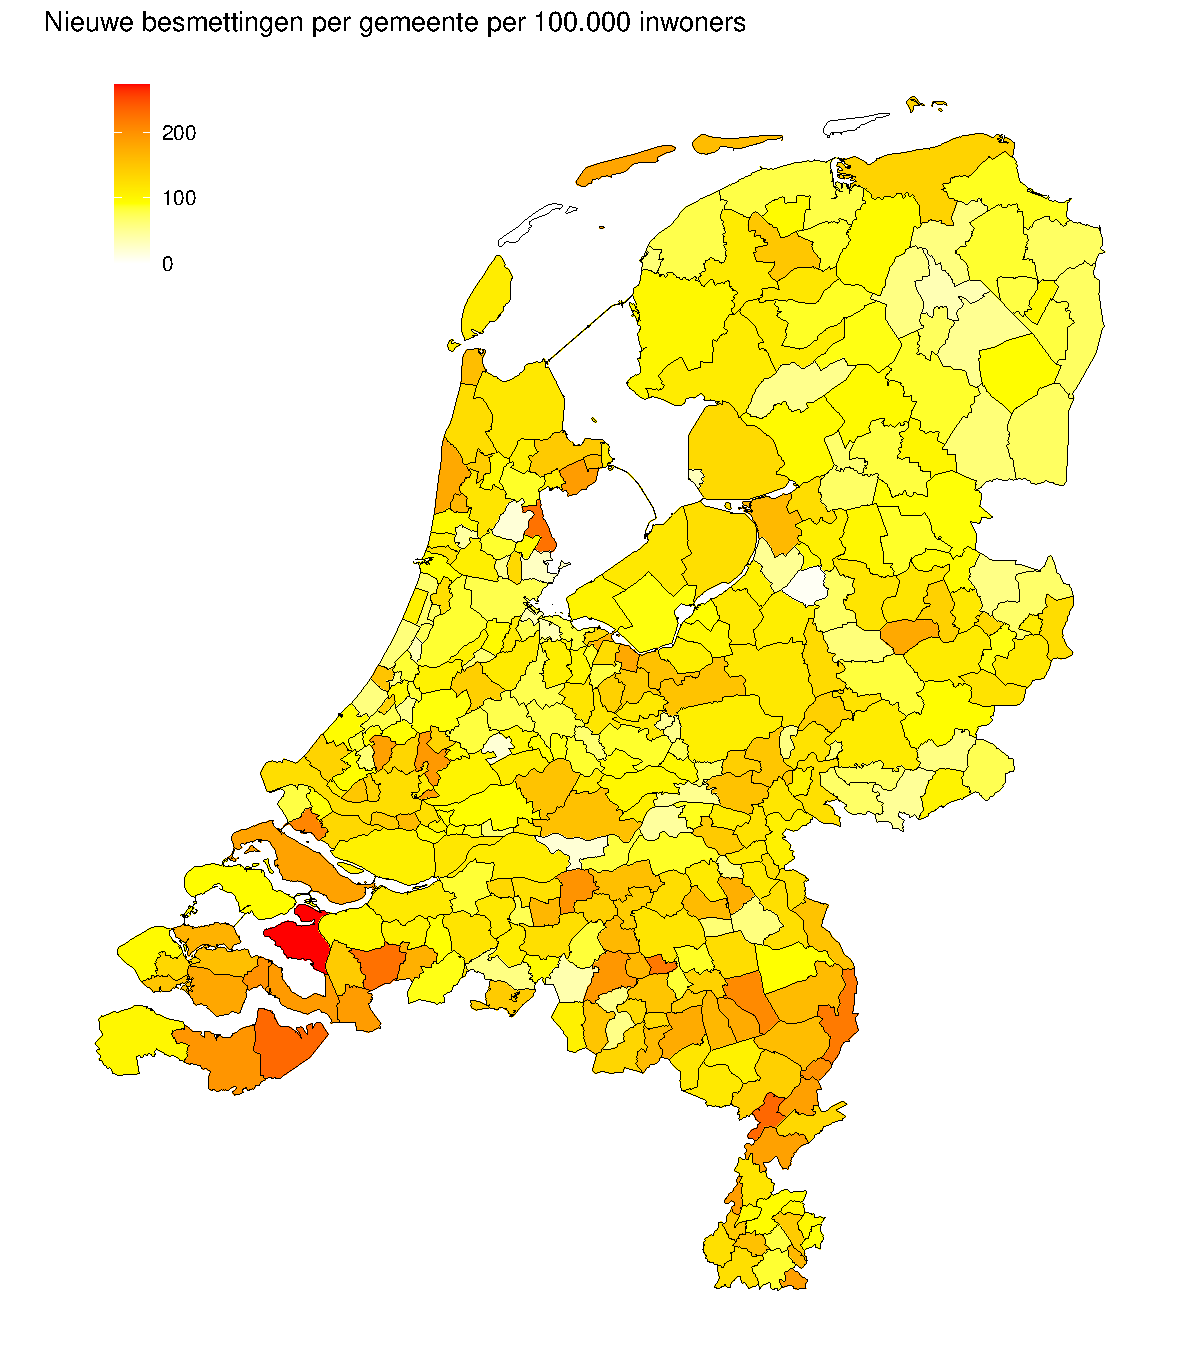
\includegraphics{daily_report_files/figure-latex/Gemeentes - sinds gisteren-1.pdf}
\caption{(\#Gemeentes - sinds gisteren) Aantal, sinds gisteren, bij de GGD'en gemelde COVID-19 patiënten per 100.000 inwoners per gemeente}
\end{figure}

\newpage

\hypertarget{kaart-met-covid-19-meldingen-per-gemeente-in-de-afgelopen-week}{%
\section{Kaart met COVID-19 meldingen per gemeente in de afgelopen week}\label{kaart-met-covid-19-meldingen-per-gemeente-in-de-afgelopen-week}}

\begin{figure}
\centering
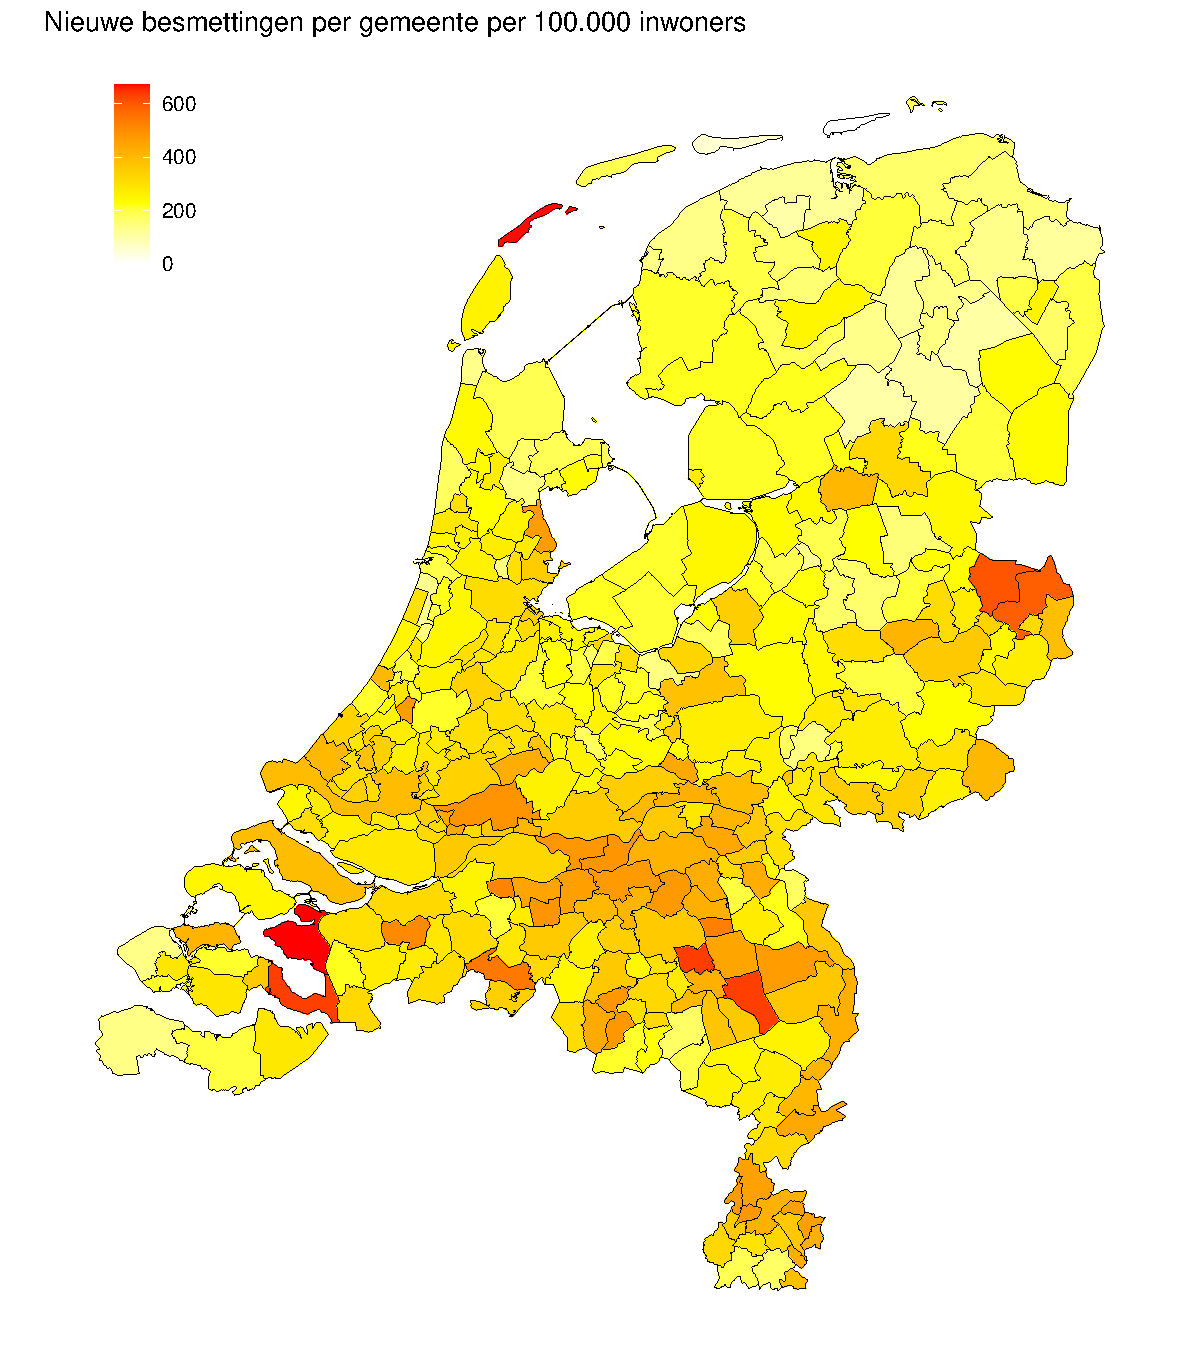
\includegraphics{daily_report_files/figure-latex/Gemeentes - Sinds vorige week-1.pdf}
\caption{(\#Gemeentes - Sinds vorige week) Aantal in de afgelopen week bij de GGD'en gemelde COVID-19 patiënten per 100.000 inwoners per gemeente.}
\end{figure}

\newpage

\hypertarget{aantal-covid-19-meldingen-per-provincie-in-de-afgelopen-twee-weken}{%
\section{Aantal COVID-19 meldingen per provincie in de afgelopen twee weken}\label{aantal-covid-19-meldingen-per-provincie-in-de-afgelopen-twee-weken}}

\begin{table}
\centering
\begin{threeparttable}
\begin{tabular}{lrrrrrr}
\toprule
\multicolumn{1}{c}{ } & \multicolumn{2}{c}{Besmettingen} & \multicolumn{2}{c}{Ziekenhuisopnames} & \multicolumn{2}{c}{Overleden} \\
\cmidrule(l{3pt}r{3pt}){2-3} \cmidrule(l{3pt}r{3pt}){4-5} \cmidrule(l{3pt}r{3pt}){6-7}
Provincie & Totaal & /100000 & Totaal & /100000 & Totaal & /100000\\
\midrule
Drenthe & 6274 & 1261.2 & 28 & 5.6 & 16 & 3.2\\
Flevoland & 6928 & 1598.3 & 33 & 7.6 & 14 & 3.2\\
Fryslân & 11440 & 1749.4 & 62 & 9.5 & 20 & 3.1\\
Gelderland & 33654 & 1596.1 & 139 & 6.6 & 144 & 6.8\\
Groningen & 6305 & 1068.6 & 33 & 5.6 & 25 & 4.2\\
Limburg & 27131 & 2425.2 & 131 & 11.7 & 98 & 8.8\\
Noord-Brabant & 47107 & 1819.0 & 152 & 5.9 & 123 & 4.7\\
Noord-Holland & 43538 & 1500.3 & 185 & 6.4 & 105 & 3.6\\
Overijssel & 17910 & 1529.7 & 59 & 5.0 & 40 & 3.4\\
Utrecht & 23329 & 1705.9 & 30 & 2.2 & 44 & 3.2\\
Zeeland & 8395 & 2170.6 & 98 & 25.3 & 16 & 4.1\\
Zuid-Holland & 58700 & 1566.6 & 228 & 6.1 & 142 & 3.8\\
\bottomrule
\end{tabular}
\begin{tablenotes}
\item \textit{Note: } 
\item Aantal bij de GGD’en gemelde COVID-19 patiënten, in het ziekenhuis opgenomen COVID-19 patiënten en overleden COVID-19 patiënten per provincie van 26 november t/m 10 december 10:00 uur, totaal en per 100.000 inwoners
\end{tablenotes}
\end{threeparttable}
\end{table}

\newpage

\hypertarget{aantal-covid-19-meldingen-per-ggd-in-de-afgelopen-twee-weken}{%
\section{Aantal COVID-19 meldingen per GGD in de afgelopen twee weken}\label{aantal-covid-19-meldingen-per-ggd-in-de-afgelopen-twee-weken}}

\begin{table}
\centering\begingroup\fontsize{10}{12}\selectfont

\begin{threeparttable}
\begin{tabular}{lrrrrrr}
\toprule
\multicolumn{1}{c}{ } & \multicolumn{2}{c}{Besmettingen} & \multicolumn{2}{c}{Ziekenhuisopnames} & \multicolumn{2}{c}{Overleden} \\
\cmidrule(l{3pt}r{3pt}){2-3} \cmidrule(l{3pt}r{3pt}){4-5} \cmidrule(l{3pt}r{3pt}){6-7}
GGD & Totaal & /100000 & Totaal & /100000 & Totaal & /100000\\
\midrule
Dienst Gezondheid \& Jeugd ZHZ & 8704 & 1878.5 & 26 & 5.6 & 37 & 8.0\\
GGD Amsterdam & 13521 & 1249.0 & 58 & 5.4 & 37 & 3.4\\
GGD Brabant-Zuidoost & 13751 & 1739.5 & 47 & 5.9 & 46 & 5.8\\
GGD Drenthe & 6293 & 1264.4 & 28 & 5.6 & 15 & 3.0\\
GGD Flevoland & 6916 & 1593.4 & 33 & 7.6 & 14 & 3.2\\
GGD Fryslân & 11459 & 1751.3 & 63 & 9.6 & 21 & 3.2\\
GGD Gelderland-Zuid & 9927 & 1746.2 & 52 & 9.1 & 32 & 5.6\\
GGD Gooi en Vechtstreek & 4332 & 1661.8 & 12 & 4.6 & 13 & 5.0\\
GGD Groningen & 6041 & 1022.6 & 31 & 5.2 & 25 & 4.2\\
GGD Haaglanden & 16299 & 1440.0 & 78 & 6.9 & 36 & 3.2\\
GGD Hart voor Brabant & 19957 & 1836.2 & 45 & 4.1 & 52 & 4.8\\
GGD Hollands-Midden & 12492 & 1523.1 & 37 & 4.5 & 22 & 2.7\\
GGD Hollands-Noorden & 11520 & 1720.6 & 51 & 7.6 & 26 & 3.9\\
GGD IJsselland & 7837 & 1457.6 & 26 & 4.8 & 21 & 3.9\\
GGD Kennemerland & 9226 & 1666.7 & 42 & 7.6 & 20 & 3.6\\
GGD Limburg-Noord & 12260 & 2338.5 & 48 & 9.2 & 42 & 8.0\\
GGD Noord- en Oost-Gelderland & 12786 & 1531.5 & 52 & 6.2 & 62 & 7.4\\
GGD Regio Utrecht & 23348 & 1705.6 & 31 & 2.3 & 45 & 3.3\\
GGD Rotterdam-Rijnmond & 21241 & 1590.8 & 87 & 6.5 & 48 & 3.6\\
GGD Twente & 10102 & 1593.9 & 32 & 5.0 & 19 & 3.0\\
GGD West-Brabant & 13459 & 1883.8 & 59 & 8.3 & 25 & 3.5\\
GGD Zaanstreek/Waterland & 4949 & 1453.4 & 25 & 7.3 & 8 & 2.3\\
GGD Zeeland & 8408 & 2173.3 & 98 & 25.3 & 16 & 4.1\\
GGD Zuid-Limburg & 14934 & 2509.3 & 82 & 13.8 & 56 & 9.4\\
Veiligheids- en Gezondheidsregio Gelderland-Midden & 10949 & 1550.0 & 35 & 5.0 & 49 & 6.9\\
\bottomrule
\end{tabular}
\begin{tablenotes}
\item \textit{Note: } 
\item Aantal bij de GGD’en gemelde COVID-19 patiënten, in het ziekenhuis opgenomen COVID-19 patiënten en overleden COVID-19 patiënten per GGD van 26 november t/m 10 december 10:00 uur, totaal en per 100.000 inwoners
\end{tablenotes}
\end{threeparttable}
\endgroup{}
\end{table}

\newpage

\hypertarget{ziekenhuisopnames-nice-in-de-afgelopen-twee-weken}{%
\section{Ziekenhuisopnames (NICE) in de afgelopen twee weken}\label{ziekenhuisopnames-nice-in-de-afgelopen-twee-weken}}

\begin{table}
\centering\begingroup\fontsize{10}{12}\selectfont

\begin{threeparttable}
\begin{tabular}{lrrrrrr}
\toprule
\multicolumn{1}{c}{ } & \multicolumn{2}{c}{Aanwezig} & \multicolumn{2}{c}{Opnames} & \multicolumn{2}{c}{Overleden} \\
\cmidrule(l{3pt}r{3pt}){2-3} \cmidrule(l{3pt}r{3pt}){4-5} \cmidrule(l{3pt}r{3pt}){6-7}
Leeftijd & Kliniek & IC & Kliniek & IC & Kliniek & IC\\
\midrule
<20 & 63 & 3 & 126 & 4 & 0 & -1\\
20 - 24 & 8 & 2 & 40 & 5 & 0 & 0\\
25 - 29 & 25 & 6 & 65 & 8 & 0 & 1\\
30 - 34 & 38 & 13 & 85 & 20 & 0 & 0\\
35 - 39 & 39 & 22 & 101 & 26 & 1 & 0\\
40 - 44 & 51 & 16 & 111 & 20 & 1 & 3\\
45 - 49 & 62 & 48 & 129 & 59 & 0 & 5\\
50 - 54 & 108 & 66 & 186 & 73 & 4 & 3\\
55 - 59 & 130 & 94 & 234 & 100 & 5 & 10\\
60 - 64 & 144 & 101 & 274 & 105 & 10 & 24\\
65 - 69 & 203 & 115 & 345 & 106 & 35 & 34\\
70 - 74 & 260 & 109 & 423 & 107 & 74 & 45\\
75 - 79 & 384 & 52 & 544 & 76 & 129 & 42\\
80 - 84 & 267 & 5 & 464 & 8 & 170 & 5\\
85 - 89 & 187 & 0 & 369 & 1 & 127 & 0\\
>90 & 97 & 0 & 174 & 0 & 56 & 0\\
\bottomrule
\end{tabular}
\begin{tablenotes}
\item \textit{Note: } 
\item Aantal bij NICE gemelde COVID-19 patiënten: in het ziekenhuis aanwezige COVID-19 patiënten, opnames, en overleden COVID-19 patiënten in het ziekenhuis van 26 november t/m 10 december 15:15 uur
\end{tablenotes}
\end{threeparttable}
\endgroup{}
\end{table}

\newpage

\hypertarget{leeftijdsverdeling-en-man-vrouwverdeling-van-covid-19-patiuxebnten-in-de-afgelopen-twee-weken}{%
\section{Leeftijdsverdeling en man-vrouwverdeling van COVID-19 patiënten in de afgelopen twee weken}\label{leeftijdsverdeling-en-man-vrouwverdeling-van-covid-19-patiuxebnten-in-de-afgelopen-twee-weken}}

\begin{table}
\centering\begingroup\fontsize{11}{13}\selectfont

\begin{threeparttable}
\begin{tabular}{lrrrrrr}
\toprule
\multicolumn{1}{c}{ } & \multicolumn{2}{c}{Besmettingen} & \multicolumn{2}{c}{Ziekenhuisopnames} & \multicolumn{2}{c}{Overleden} \\
\cmidrule(l{3pt}r{3pt}){2-3} \cmidrule(l{3pt}r{3pt}){4-5} \cmidrule(l{3pt}r{3pt}){6-7}
Leeftijdsgroep & Totaal & \% & Totaal & \% & Totaal & \%\\
\midrule
<50 & 9 & 0.0 & 5 & 0.4 & 9 & 1.1\\
0-9 & 40670 & 14.0 & 37 & 3.1 & NA & NA\\
10-19 & 45896 & 15.8 & 7 & 0.6 & NA & NA\\
20-29 & 33377 & 11.5 & 13 & 1.1 & NA & NA\\
30-39 & 45117 & 15.5 & 36 & 3.1 & NA & NA\\
40-49 & 42691 & 14.7 & 63 & 5.3 & NA & NA\\
50-59 & 32120 & 11.0 & 131 & 11.1 & 16 & 2.0\\
60-69 & 24879 & 8.6 & 212 & 18.0 & 45 & 5.7\\
70-79 & 15330 & 5.3 & 357 & 30.3 & 160 & 20.3\\
80-89 & 8203 & 2.8 & 273 & 23.2 & 370 & 47.0\\
90+ & 2419 & 0.8 & 44 & 3.7 & 187 & 23.8\\
\bottomrule
\end{tabular}
\begin{tablenotes}
\item[1] Leeftijdsverdeling van bij de GGD’en gemelde COVID-19 patiënten, in het ziekenhuis opgenomen COVID-19 patiënten en overleden COVID-19 patiënten van 26 november t/m 10 december 10:00 uur.
\item[2] Overlijdensgevallen van patiënten jonger dan 50 jaar oud worden door het RIVM in de casusdata gegroepeerd in de categorie <50. Deze overlijdensgevallen zijn hier dus niet zichtbaar in deze leeftijdsgroepen maar alleen via de groep '<50'.
\end{tablenotes}
\end{threeparttable}
\endgroup{}
\end{table}

\newpage

\begin{table}
\centering\begingroup\fontsize{11}{13}\selectfont

\begin{threeparttable}
\begin{tabular}{lrrrrrr}
\toprule
\multicolumn{1}{c}{ } & \multicolumn{2}{c}{Besmettingen} & \multicolumn{2}{c}{Ziekenhuisopnames} & \multicolumn{2}{c}{Overleden} \\
\cmidrule(l{3pt}r{3pt}){2-3} \cmidrule(l{3pt}r{3pt}){4-5} \cmidrule(l{3pt}r{3pt}){6-7}
Geslacht & Totaal & \% & Totaal & \% & Totaal & \%\\
\midrule
Vrouw & 151049 & 52 & 483 & 41 & 376 & 47.8\\
Man & 139662 & 48 & 695 & 59 & 411 & 52.2\\
Onbekend & 0 & 0 & 0 & 0 & NA & NA\\
\bottomrule
\end{tabular}
\begin{tablenotes}
\item \textit{Note: } 
\item Man-vrouwverdeling van bij de GGD’en gemelde COVID-19 patiënten, in het ziekenhuis opgenomen COVID-19 patiënten en overleden COVID-19 patiënten van 26 november t/m 10 december 10:00 uur.
\end{tablenotes}
\end{threeparttable}
\endgroup{}
\end{table}
\newpage


\end{document}
